\documentclass[12pt]{article}
\usepackage{graphicx}

%%% margins 
\textheight 23.4cm
\textwidth 14.65cm
\oddsidemargin 0.375in
\evensidemargin 0.375in
\topmargin  -0.55in

\begin{document}
  \begin{figure}
    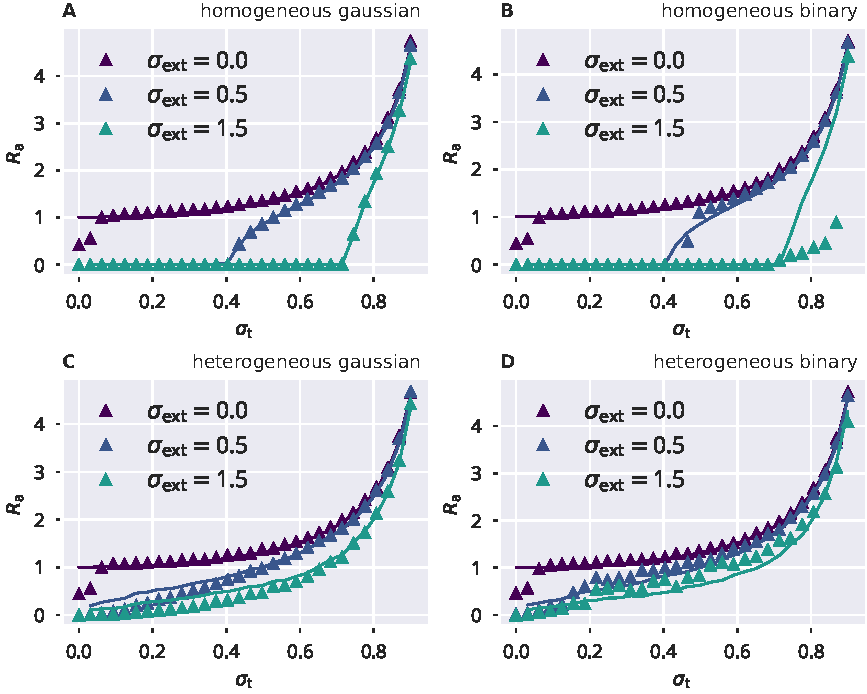
\includegraphics[width=5.78in]{./r_a_sweep_composite.pdf}
    \label{fig:alt_hom_regulation}
    \caption{ $R_{\rm a}$ for different external input variances. Lines show the exact solution of \{reference to gaussian integral equation\}, markers are full network simulations.
    {\bf A}: Homogeneous independent gaussian input.
     {\bf B}: Homogeneous identical binary input. 
     {\bf C}: Heterogeneous independent gaussian input. 
     {\bf D}: Heterogeneous identical binary input.}
  \end{figure}
\end{document}